\documentclass[12pt,a4paper]{article}

\usepackage[margin=2.5cm]{geometry}
\usepackage{amsmath,amssymb,amsthm}
\usepackage{mathtools}
\usepackage{booktabs}
\usepackage{array}
\usepackage{graphicx}
\usepackage{float}
\usepackage{caption}
\usepackage{subcaption}
\usepackage{placeins}
\usepackage{enumitem}
\usepackage{mathpazo}
\usepackage[T1]{fontenc}
\usepackage[utf8]{inputenc}
\usepackage[british]{babel}
\usepackage{microtype}
\usepackage[dvipsnames]{xcolor}
\usepackage[colorlinks=true,linkcolor=ForestGreen,citecolor=ForestGreen,urlcolor=ForestGreen]{hyperref}

\captionsetup{labelfont=normalfont,font=small,skip=4pt}
\setlength{\parindent}{0pt}
\setlength{\parskip}{0.7em}
\setlength{\emergencystretch}{2em}
\setcounter{secnumdepth}{2}
\renewcommand{\thesubsection}{\thesection\alph{subsection}}
\graphicspath{{output/}}

\newcommand{\probsection}[2]{\section{#2}}
\newcommand{\probsub}[2]{\subsection{#2}}
\newcommand{\code}[1]{\texttt{#1}}
\newcommand{\Me}{\mathrm{Me}}
\newcommand{\BH}{\mathrm{BH}}
\newcommand{\ev}{\mathrm{ev}}

% Reported figures, generated from output/ by make_macros.py. The prose cites
% these macros so every number is defined once, from the data.
% Generated by make_macros.py -- do not edit by hand.
% Each value is read from output/ at report precision.

\newcommand{\DBlsCumRet}{1.31}
\newcommand{\DBlsExcess}{2.00}
\newcommand{\DBlsSharpe}{237}
\newcommand{\DBlsAnnVol}{0.45}
\newcommand{\DBlsMaxDD}{-0.38}
\newcommand{\DBlsDDLen}{123}
\newcommand{\DBlsTrades}{45}
\newcommand{\DBbhCumRet}{-0.70}
\newcommand{\DBbhLossPct}{70}
\newcommand{\DBloExcessPts}{80}
\newcommand{\DBrollExcessMean}{0.819}
\newcommand{\DBrollExcessStd}{0.216}
\newcommand{\DBrollWindows}{347}
\newcommand{\DBrollHalfExcessMean}{0.383}
\newcommand{\HSlsCumRet}{0.55}
\newcommand{\HSlsExcess}{1.17}
\newcommand{\HSlsTrades}{46}
\newcommand{\HSlsMaxDD}{-0.11}
\newcommand{\HSbhCumRet}{-0.61}
\newcommand{\HSbhLossPct}{61}
\newcommand{\HSrollExcessMean}{0.294}
\newcommand{\HSrollWinPct}{57}
\newcommand{\HSloWinPct}{0.59}
\newcommand{\HSloExcessWin}{0.47}
\newcommand{\DBruleOnHS}{0.71}
\newcommand{\HSruleOnDB}{1.35}
\newcommand{\DBwfMean}{0.20}
\newcommand{\HSwfMean}{0.11}
\newcommand{\DBwfCrash}{0.82}
\newcommand{\HSwfCrash}{0.72}
\newcommand{\wfTrainLo}{0.2}
\newcommand{\wfTrainHi}{1.3}
\newcommand{\AmPuts}{522}
\newcommand{\AmCalls}{478}
\newcommand{\AmNumMs}{6.3}
\newcommand{\BaNumMs}{18.9}
\newcommand{\BaSEmean}{0.083}
\newcommand{\BaSEpHi}{0.137}
\newcommand{\BaGPRmae}{0.122}
\newcommand{\BaMonoGPR}{74}
\newcommand{\BaMonoNN}{76}
\newcommand{\AmGPRbe}{5{,}100}
\newcommand{\AmNNbe}{530}
\newcommand{\BaGPRbe}{5{,}100}
\newcommand{\BaNNbe}{100}
\newcommand{\BSMref}{11.348}
\newcommand{\EulerErrVone}{+0.231}
\newcommand{\EulerErrVtwo}{+0.065}
\newcommand{\HesScalarMs}{518}
\newcommand{\HesScaledMs}{5{,}200}
\newcommand{\HesVecMs}{31}


\makeatletter
\renewcommand{\maketitle}{%
  \begin{center}
  {\Large \@title\par}
  \vspace{0.35em}
  {\fontsize{11pt}{13.2pt}\selectfont \@author\par}
  \vspace{0.15em}
  {\@date\par}
  \end{center}
  \vspace{0.7em}}
\makeatother

\title{Homework 2: Machine Learning for Finance}
\author{Marco Canal, Michael Duarte Gonçalves and Olivia Peter}
\date{17 June 2026}

\begin{document}
\maketitle
\vspace{0.2em}

\section{Backtesting trading strategies on sentiment indicators}

The sentiment columns in \texttt{dataSent} can be read as daily,
target-specific sentiment indicators. At the document
level a lexicon-based score for target $G_k$ is
$S_{n,t}(\lambda,k)=\sum_i w_i\,S_{i,n,t}(\lambda,k)$ and the daily indicator
is the aggregation $S_t(\lambda,k)=\sum_{n=1}^{N_t}\beta_n\,S_{n,t}(\lambda,k)$
over the $N_t$ timestamped documents of day $t$. Here $\lambda$ selects the
sentiment lexicon and $k$ the target, $i$ runs over the unigrams of document $n$
with weights $w_i$, $S_{i,n,t}$ is the lexicon value of unigram $i$ and
$\beta_n$ weights each document in the daily total. We therefore treat
positiveP, negativeP, certaintyP, uncertaintyP, finupP and findownP as
observed daily sentiment series for each stock and build the assignment
indicators as transformations of them. These columns are aggregated sentiment
measures with an economic meaning rather than arbitrary numbers, which is what
gives the transformations below their interpretation.

Our two stocks are Deutsche Bank (DB) and HSBC. Both are international banks and
both saw their adjusted-close series in \texttt{dataSent} fall sharply from
January~2018 to May~2020. We flag this now because it sets a low buy-and-hold
bar, a point we come back to when reading the results.

\subsection{Indicators}
Each daily file runs from 2~January~2018 to 22~May~2020 and supplies, beside the
OHLC record, the percentage-tone scores and the news-volume measure RVT. From
the tone scores we construct
\begin{gather*}
\mathrm{BULL} = \mathrm{positiveP} + \mathrm{certaintyP} + \mathrm{finupP}, \\
\mathrm{BEAR} = \mathrm{negativeP} + \mathrm{uncertaintyP} + \mathrm{findownP},
\end{gather*}
\[
\mathrm{BBr} = \frac{100\,\mathrm{BULL}}{\mathrm{BULL} + \mathrm{BEAR}},
\qquad
\mathrm{PNlog} = \tfrac{1}{2}\log\!\left(\frac{\mathrm{positiveP} + 1}{\mathrm{negativeP} + 1}\right).
\]
On the rare days where both BULL and BEAR are zero the ratio BBr is undefined.
We fill those gaps by forward fill after the first valid observation so that no
future information leaks back into the early sample. The explanatory-variable
catalogue used in tuning is
$\ev \in \{\mathrm{positiveP}, \mathrm{negativeP}, \mathrm{BULL}, \mathrm{BEAR},
\mathrm{BBr}, \mathrm{PNlog}\}$, with RVT held aside as the confirmation source.

\subsection{The signal}
Our signalling rule is a sentiment slope confirmed by a news-volume z-score.
Given a slope lag $L$, an RVT window $W$ and a confirmation threshold $\tau$,
the $L$-day change in the explanatory variable is
$\mathrm{slope}_t = \ev_t - \ev_{t-L}$ and the standardised news volume is
\[
z_t = \frac{\mathrm{RVT}_t - \mu^{\mathrm{RVT}}_t}{\sigma^{\mathrm{RVT}}_t},
\qquad
\mu^{\mathrm{RVT}}_t = \mathrm{mean}_{t-W:t}(\mathrm{RVT}),\quad
\sigma^{\mathrm{RVT}}_t = \mathrm{std}_{t-W:t}(\mathrm{RVT}).
\]
The decision at $t$ is to go long when the slope is positive and $|z_t|>\tau$,
to exit (flat in the long-only regime, weight $-1$ in the long-short regime)
when the slope is negative and $|z_t|>\tau$ and to hold otherwise. We lag the
signal one day, so the trade at $t+1$ uses only information through $t$. Both
conditions must hold together, so a tone change moves the position only after a
burst of news confirms it.

Two stylised facts about news sentiment motivate this. The first is that news
volume and volatility move together, so a tone change arriving on abnormal news
flow is likelier to carry information than a quiet drift in the score. The
second is asymmetry. Bad news tracks market moves more tightly than good news,
which is why the rule will exit or short when the slope deteriorates under heavy
news flow. Quiet wiggles in tone are mostly noise. Once the 1\% cost is paid on
every flip, trading them loses money. The volume filter is there so we act only
when the news is genuinely moving.

\subsection{Tuning}
The free parameters are the slope lag $L\in\{5,10,20\}$, the RVT window
$W\in\{20,40\}$, the threshold $\tau\in\{0,0.5,1\}$, the choice of $\ev$ and the
long-short flag. We select them by grid search over the whole sample,
maximising the cumulative excess return $\Me_T-\BH_T$ subject to a floor of
five trades. The floor removes degenerate configurations that almost never trade
and would otherwise score well simply by sitting out a falling benchmark. We also ran three other sentiment families during development,
Bollinger bands, MACD and a rolling-percentile breakout on $\ev$. The
slope-with-confirmation family held up best across both banks and it is the
one we submit.

We score the grid on the same period we then report on, so the headline tables
are \emph{in-sample model selection} followed by descriptive rolling
diagnostics, not out-of-sample validation. The guard against overfitting holds
only in part. The same family and the same timing, $L=W=20$ and $\tau=1$, are
picked for both banks and only the explanatory variable differs, BBr for DB and
positiveP for HSBC. A stricter test freezes one bank's whole configuration and
runs it unchanged on the other. That still clears buy-and-hold after costs: the
DB rule earns a cumulative excess of $\DBruleOnHS$ on HSBC and the HSBC rule
earns $\HSruleOnDB$ on DB. To remove the hindsight altogether we also run a walk-forward
test, which fixes the parameters on data before each evaluation window. It is
reported in Section~\ref{sec:walkforward} and is the out-of-sample check.

\subsection{Conventions}
We measure performance by the excess return after costs. A completed
long-only buy-sell trade from day $b$ to day $s$ has
log return $r_{bs}=\log(P_s/P_b)-2C$, where $P_b$ and $P_s$ are the buy and sell
prices and $C$ is the one-way cost. For a rule $\rho$ the period return is
$r=\sum_{t} I_\rho(t)\,r_t - 2nC$, where $I_\rho(t)$ is one on the days the rule
is invested, $r_t$ is the day-$t$ return and $n$ is the number of completed
trades. Buy-and-hold is $r_{1T}=\log(P_T/P_1)-2C$ with $P_1$ and $P_T$ the first
and last prices. The headline figure is the excess
$\Me-\BH=r-r_{1T}$. We charge the cost once per position change at the rate
$C=0.01$, so the total cost over a window is (number of position
changes)$\times 0.01$ taken off the cumulative return. A direct long-to-short
flip therefore counts as a single position change, handled the same way for
whole-period and rolling results. Two of the metrics need a precise definition:
\begin{enumerate}[label=\roman*., itemsep=1pt]
  \item \emph{Sharpe.} We report the Sharpe ratio as an annualised return over
  daily volatility scaled by $\sqrt{252}$. That scaling inflates it by a factor
  of $252$ over the conventional reward-to-variability ratio
  $SR=(E(R)-r_f)/\operatorname{std}(R)$, with $r_f$ set to zero, so the values
  run into the hundreds and are best read as relative rankings rather than
  standard Sharpe numbers.
  \item \emph{Maximum drawdown.} We define it as the worst peak-to-trough drop
  of the cumulative-return path, $\min_t\,(\mathrm{cum}_t-\max_{s\le t}\mathrm{cum}_s)$,
  with the drawdown length the longest stretch the path spends below a prior
  peak. We compute that length directly as the longest underwater run, so the
  values reported below are non-zero.
\end{enumerate}

\subsection{In-sample results}
Deutsche Bank and HSBC are tuned and evaluated the same way, so we report them
together. The whole-period and rolling tables below are the in-sample
selection, scored on the same period we tuned on; the out-of-sample check is the
walk-forward of Section~\ref{sec:walkforward}.

\paragraph{Deutsche Bank.}
The tuned configuration is $\ev=\mathrm{BBr}$, $L=W=20$ days, $\tau=1.0$.
Table~\ref{tab:db_whole} gives the whole-period metrics. In long-short form the
strategy returns a cumulative $\DBlsCumRet$ against a buy-and-hold of
$\DBbhCumRet$ over the $2.5$-year sample, an excess of $\DBlsExcess$ after the
cost on each of its $\DBlsTrades$ trades. Its Sharpe is $\DBlsSharpe$ on this
scaling, its annualised volatility $\DBlsAnnVol$ and its worst drawdown
$\DBlsMaxDD$ lasting $\DBlsDDLen$ trading days. The long-only version still
beats buy-and-hold by $\DBloExcessPts$ points of cumulative
return, just by standing aside on weak-sentiment days. So a good part of the
edge is staying out when the news turns bad, not the short leg alone.

\begin{table}[ht]
\centering
\scriptsize
\setlength{\tabcolsep}{4pt}
\begin{tabular}{lrrrrrrrr}
\toprule
configuration & CumRet & AnnRet & Sharpe & WinPct & AnnVol & MaxDD & DDLen & nTrades \\
\midrule
DB long-short   &  1.306 &  0.420 &  236.8 & 0.541 & 0.447 & $-0.382$ & 123 & 45 \\
DB long-only    &  0.104 &  0.042 &   40.6 & 0.521 & 0.263 & $-0.262$ & 258 & 44 \\
DB buy-and-hold & $-0.699$ & $-0.395$ & $-219.9$ & 0.480 & 0.453 & $-1.071$ & 586 & 1 \\
\bottomrule
\end{tabular}
\caption{Whole-period DB metrics for the long-short and long-only rules against
buy-and-hold (BBr, $L=W=20$, $\tau=1.0$), net of the 1\% cost.}
\label{tab:db_whole}
\end{table}

Table~\ref{tab:db_rolling} reports the rolling-window analysis. At one-year
windows the long-short configuration averages a positive excess of
$\DBrollExcessMean$ per window with a window-by-window standard deviation of
$\DBrollExcessStd$ and it beats
buy-and-hold in every one of the $\DBrollWindows$ overlapping windows. The six-month
windows hold up at a shorter horizon, with a mean excess of
$\DBrollHalfExcessMean$ and even the long-only configurations stay positive in
mean excess at
both lengths. Trade counts scale as expected, around $20$ a year and $10$ a
half-year, so the cost base stays modest relative to the gain. The
$\DBrollWindows$ one-year windows overlap heavily and are far from independent
experiments, so the perfect ExcessWin record describes the chosen in-sample rule
across subperiods rather than $\DBrollWindows$ independent tests. ExcessWin is not
WinPct. WinPct counts positive days inside a window while ExcessWin counts the
windows that beat the benchmark, so the two can diverge.
The distribution of per-window excess is shown in Figure~\ref{fig:db_dist}.

\begin{table}[ht]
\centering
\scriptsize
\setlength{\tabcolsep}{3pt}
\begin{tabular}{lrrrrrrrrrr}
\toprule
configuration & windows & exc.\ mean & exc.\ std & AnnRet & AnnVol & Sharpe & WinPct & ExcessWin & MaxDD & DDLen \\
\midrule
$w{=}254$, long-short & 347 & $+0.819$ & 0.216 & $+0.542$ & 0.392 & 338.7 & 0.536 & 1.000 & $-0.300$ & 89.0 \\
$w{=}254$, long-only  & 347 & $+0.312$ & 0.119 & $+0.039$ & 0.285 & 13.7 & 0.513 & 1.000 & $-0.228$ & 124.7 \\
$w{=}127$, long-short & 474 & $+0.383$ & 0.321 & $+0.670$ & 0.391 & 380.4 & 0.531 & 0.920 & $-0.219$ & 49.3 \\
$w{=}127$, long-only  & 474 & $+0.141$ & 0.169 & $+0.076$ & 0.277 & 14.0 & 0.507 & 0.814 & $-0.160$ & 64.9 \\
\bottomrule
\end{tabular}
\caption{DB rolling-window metrics at one-year and six-month windows, 1\% cost
per window; the long-short rule beats buy-and-hold in every one-year window.}
\label{tab:db_rolling}
\end{table}

% End page 3 on the Deutsche Bank tables, then open the next page with the
% full-size histogram capping the DB discussion ahead of the HSBC paragraph.
\clearpage

\begin{figure}[t]
\centering
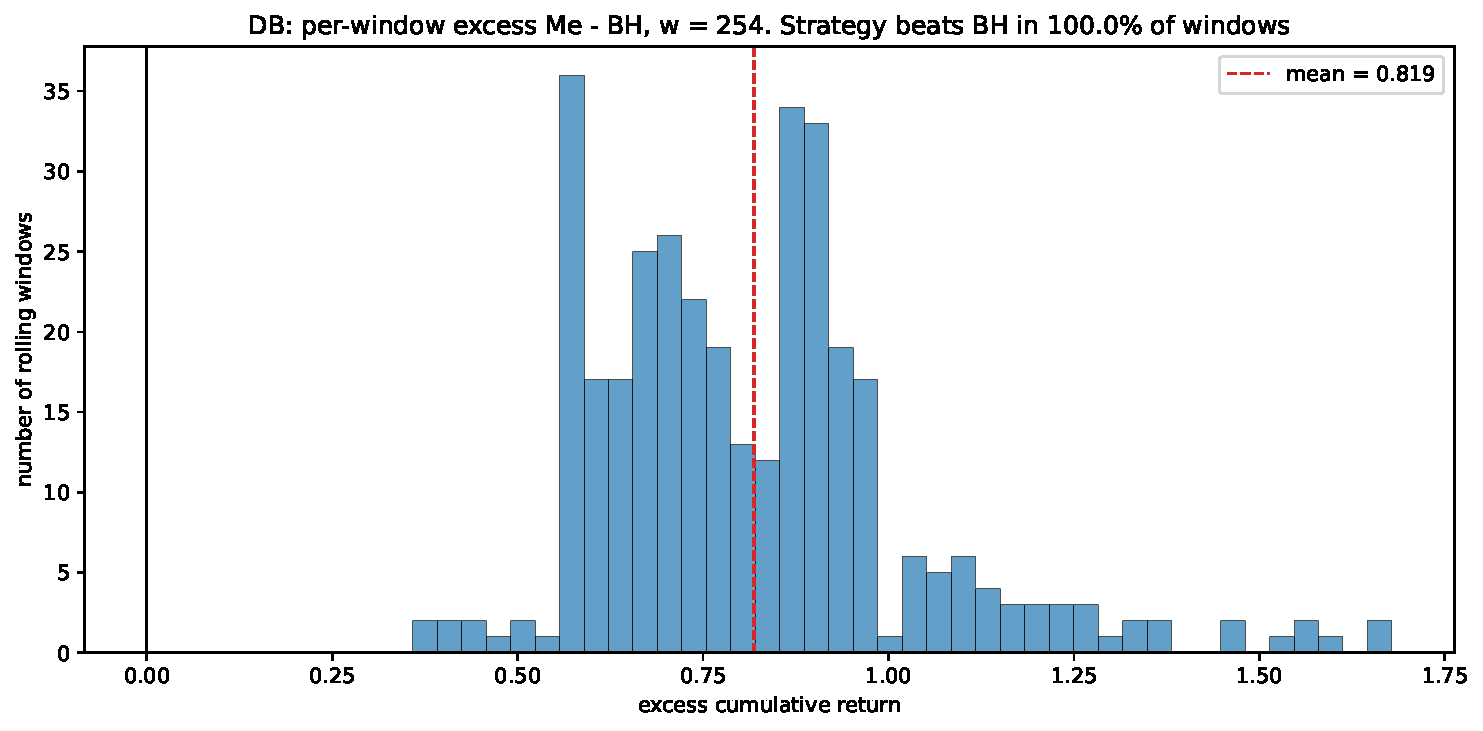
\includegraphics[width=0.92\textwidth]{ex1/figures/02_rolling_dist_DB.pdf}
\caption{DB long-short per-window excess $\Me-\BH$ over the one-year rolling
windows; every window is positive, with a right tail from the March~2020 drawdown.}
\label{fig:db_dist}
\end{figure}

\paragraph{HSBC.}
The tuned configuration is the same family with $\ev=\mathrm{positiveP}$,
$L=W=20$ and $\tau=1.0$. Only the explanatory variable changes, from the
bull-bear ratio to the positive-tone score. Table~\ref{tab:hsbc_whole} reports
the whole-period metrics: a long-short cumulative return of $\HSlsCumRet$
against a buy-and-hold of $\HSbhCumRet$, an excess of $\HSlsExcess$ after
$\HSlsTrades$ trades, with a worst drawdown of $\HSlsMaxDD$. The rolling
analysis in Table~\ref{tab:hsbc_rolling} gives a positive mean excess of
$\HSrollExcessMean$ at one-year windows with a $\HSrollWinPct\%$ win rate,
again steady across window length and the long-short flag. The six-month
long-only case shows how the two win measures can diverge. It wins on most days
(WinPct $\HSloWinPct$) yet clears buy-and-hold in under half the windows
(ExcessWin $\HSloExcessWin$).

\begin{table}[ht]
\centering
\scriptsize
\setlength{\tabcolsep}{4pt}
\begin{tabular}{lrrrrrrrr}
\toprule
configuration & CumRet & AnnRet & Sharpe & WinPct & AnnVol & MaxDD & DDLen & nTrades \\
\midrule
HSBC long-short   &  0.552 &  0.202 &  224.9 & 0.563 & 0.227 & $-0.111$ & 186 & 46 \\
HSBC long-only    & $-0.268$ & $-0.122$ & $-259.9$ & 0.553 & 0.119 & $-0.151$ & 329 & 45 \\
HSBC buy-and-hold & $-0.613$ & $-0.329$ & $-361.0$ & 0.490 & 0.229 & $-0.674$ & 591 & 1 \\
\bottomrule
\end{tabular}
\caption{Whole-period HSBC metrics (positiveP, $L=W=20$, $\tau=1.0$), net of the
1\% cost; columns as in Table~\ref{tab:db_whole}.}
\label{tab:hsbc_whole}
\end{table}

\begin{table}[ht]
\centering
\scriptsize
\setlength{\tabcolsep}{3pt}
\begin{tabular}{lrrrrrrrrrr}
\toprule
configuration & windows & exc.\ mean & exc.\ std & AnnRet & AnnVol & Sharpe & WinPct & ExcessWin & MaxDD & DDLen \\
\midrule
$w{=}254$, long-short & 347 & $+0.294$ & 0.347 & $+0.172$ & 0.181 & 222.7 & 0.574 & 0.744 & $-0.084$ & 97.7 \\
$w{=}254$, long-only  & 347 & $+0.047$ & 0.169 & $-0.073$ & 0.105 & $-149.1$ & 0.591 & 0.582 & $-0.088$ & 131.8 \\
$w{=}127$, long-short & 474 & $+0.170$ & 0.234 & $+0.222$ & 0.183 & 289.4 & 0.571 & 0.637 & $-0.071$ & 51.8 \\
$w{=}127$, long-only  & 474 & $+0.034$ & 0.115 & $-0.077$ & 0.106 & $-139.5$ & 0.592 & 0.473 & $-0.064$ & 63.6 \\
\bottomrule
\end{tabular}
\caption{HSBC rolling-window metrics; all four configurations are positive in
mean excess. Columns as in Table~\ref{tab:db_rolling}.}
\label{tab:hsbc_rolling}
\end{table}

\paragraph{Comparison.}
The two equity curves (Figures~\ref{fig:db_equity} and~\ref{fig:hsbc_equity})
behave alike, with DB the stronger case. Both strategies clear a falling
benchmark after costs: DB finishes near $+\DBlsCumRet$ against an own loss of
about $\DBbhLossPct\%$ and HSBC ends near $+\HSlsCumRet$ against about
$\HSbhLossPct\%$, excesses of $\DBlsExcess$ and $\HSlsExcess$. The DB curve sits
above its benchmark almost from the start and pulls away during the March~2020
sell-off, when the short leg profits from DB falling further. The HSBC curve
drifts around its benchmark through 2018 and 2019, then pulls clear as HSBC
collapses in early 2020. In both the edge comes mostly from sidestepping the
worst stretches and shorting into them, which is why the curves separate most
sharply in the COVID quarter.

% Both equity curves share one float so the DB and HSBC strategies stay on the
% same page, read as a pair; the \FloatBarrier below then holds every Section 1
% exhibit ahead of the walk-forward test.
\begin{figure}[ht]
\centering
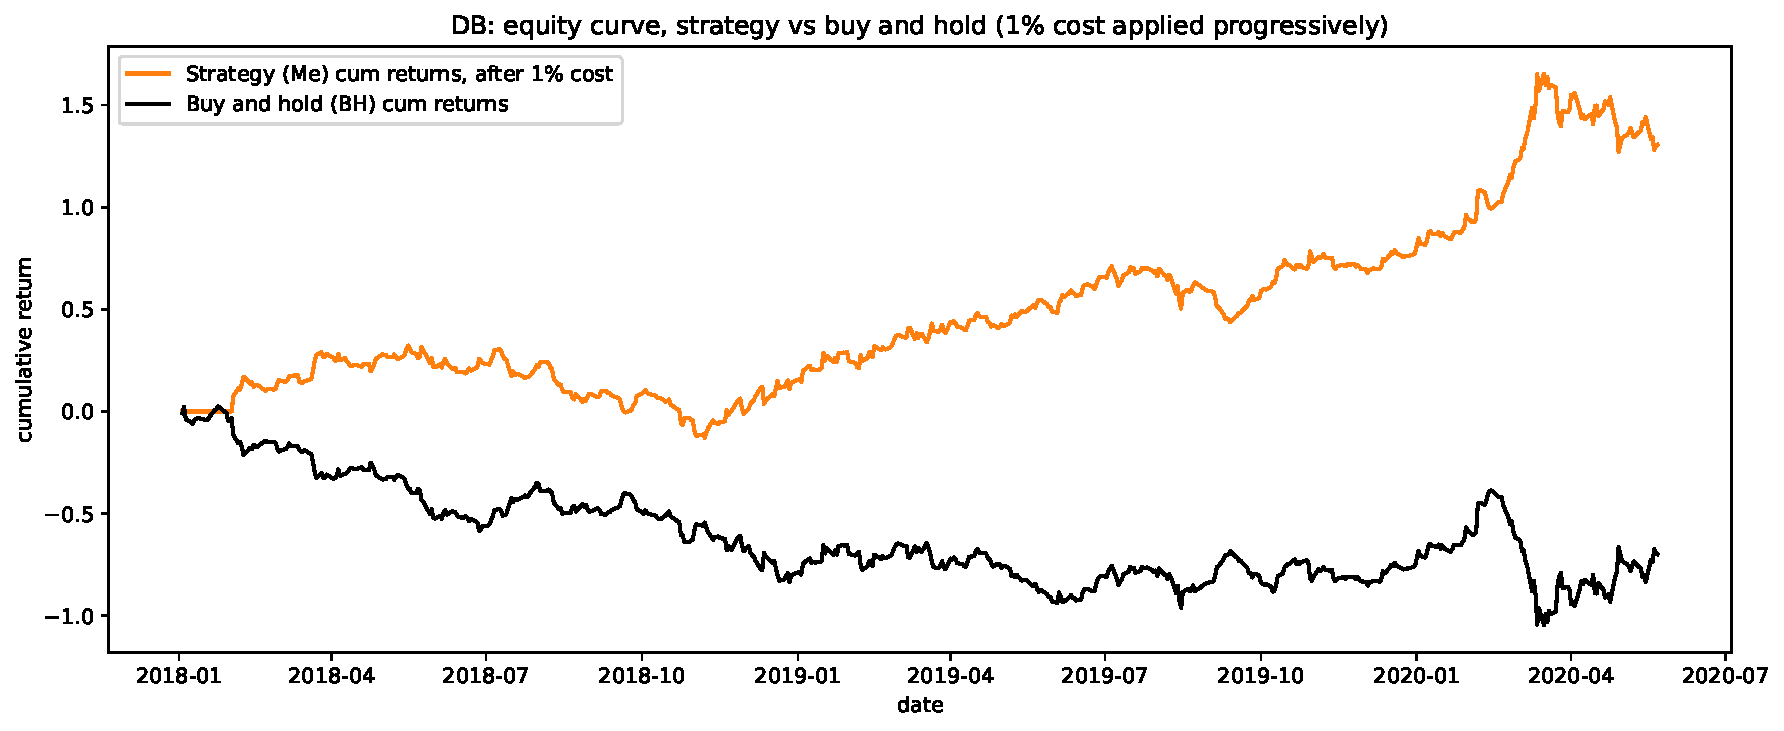
\includegraphics[width=0.92\textwidth]{ex1/figures/01_equity_DB.pdf}
\caption{DB cumulative return, strategy versus buy-and-hold with the 1\% cost
applied progressively; the long-short rule ends near $+\DBlsCumRet$.}
\label{fig:db_equity}

\vspace{1.5em}
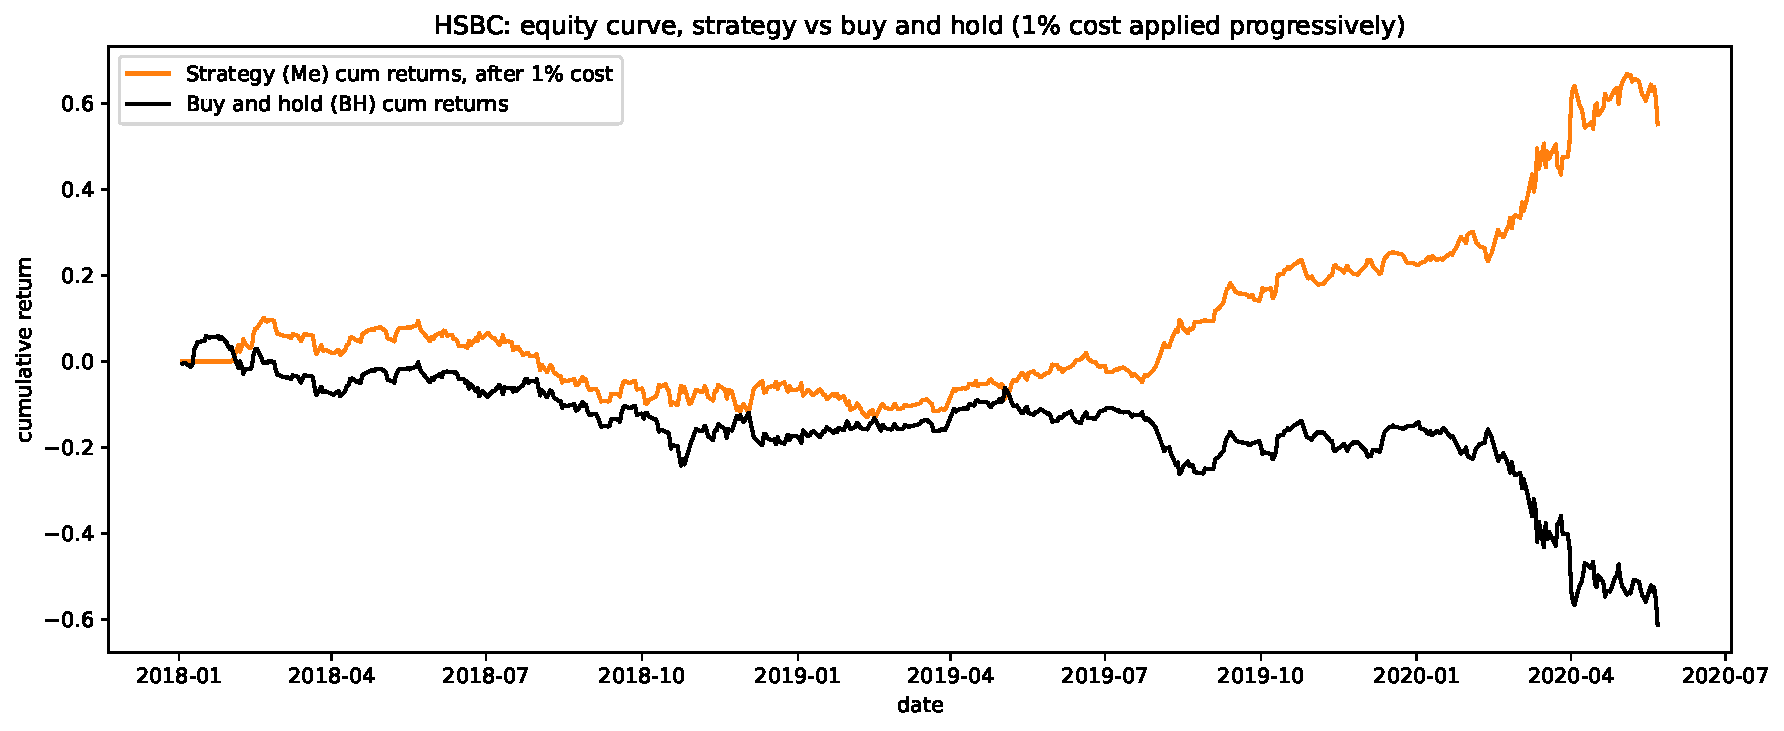
\includegraphics[width=0.92\textwidth]{ex1/figures/01_equity_HSBC.pdf}
\caption{HSBC cumulative return, strategy versus buy-and-hold with the 1\% cost
applied progressively; the strategy ends near $+\HSlsCumRet$.}
\label{fig:hsbc_equity}
\end{figure}

\FloatBarrier
\subsection{Walk-forward validation}\label{sec:walkforward}
The rolling tables still pick the rule with hindsight, because the grid is
scored on the whole sample. A stricter and more realistic test is walk-forward,
which is close to how a trading desk would actually run a signal. We tune the
rule on a block of past data, here one year, freeze it and then measure it on
the next three months that the tuning never saw. We then slide the whole window
forward and repeat. Each test quarter is out-of-sample, because its
parameters were fixed before that quarter happened.

Table~\ref{tab:walkforward} shows the result for both banks across 2019 and the
first quarter of 2020. The result is weaker than the in-sample one. On DB
the refitted rule beats buy-and-hold after costs in four of the five test
quarters, with a mean test excess of $\DBwfMean$. On HSBC it wins in only two of
five, with a mean of $\HSwfMean$. In both cases the average leans almost
entirely on one quarter, January to April 2020, when the short leg caught the
COVID crash and made $\DBwfCrash$ on DB and $\HSwfCrash$ on HSBC. Take that quarter out and the
out-of-sample edge is small on DB and slightly negative on HSBC.

The gap between train and test is the informative part. The tuner does not always choose
the submitted slope-with-confirmation rule. In the calmer quarters it often
prefers a Bollinger or percentile rule on a different sentiment variable, which
tells us no single configuration is reliably best once we stop looking at the
answer. The train excess, between $\wfTrainLo$ and $\wfTrainHi$, dwarfs the test
excess of a few percent. That gap is the overfitting the in-sample tables cannot
show. The signal has a modest regime-dependent edge and most of the headline
performance is in-sample selection rather than a repeatable out-of-sample return.

\begin{table}[ht]
\centering
\footnotesize
\setlength{\tabcolsep}{5pt}
\begin{tabular}{lllrrr}
\toprule
ticker & test quarter & tuned rule & train exc. & test exc. & nTrades \\
\midrule
DB   & 2019 Q1 & Boll/PNlog       & 1.29 & $+0.03$ & 2 \\
DB   & 2019 Q2 & Boll/PNlog       & 0.86 & $+0.08$ & 2 \\
DB   & 2019 Q3 & Slope/BBr        & 0.68 & $-0.03$ & 1 \\
DB   & 2019 Q4 & Slope/BBr        & 0.86 & $+0.09$ & 5 \\
DB   & 2020 Q1 & Slope/BBr        & 0.59 & $+0.82$ & 1 \\
\addlinespace
HSBC & 2019 Q1 & Boll/PNlog       & 0.35 & $-0.11$ & 1 \\
HSBC & 2019 Q2 & Pctile/positiveP & 0.20 & $0.00$  & 0 \\
HSBC & 2019 Q3 & Boll/BBr         & 0.20 & $+0.10$ & 3 \\
HSBC & 2019 Q4 & Pctile/positiveP & 0.40 & $-0.14$ & 4 \\
HSBC & 2020 Q1 & Slope/positiveP  & 0.27 & $+0.72$ & 2 \\
\bottomrule
\end{tabular}
\caption{Walk-forward out-of-sample test: each rule is tuned on the prior year
and frozen, then scored on the next quarter (test exc., excess after the 1\%
cost); both banks lean on the March~2020 quarter.}
\label{tab:walkforward}
\end{table}

\subsection{Discussion}
On DB and HSBC alike the signal clears buy-and-hold after costs. That holds at
the one-year and the six-month window and whether or not we allow shorting.
Both banks lost heavily over 2018 to 2020. The buy-and-hold bar is low, so any
rule that sidesteps the worst stretches starts ahead and the short leg adds to
that by catching the March~2020 crash. The confirmation filter also keeps us
out when the news is quiet. That holds trading to about $20$ a year and stops
the 1\% cost from eating the signal.

We would not over-read it. This is two correlated bank stocks
over two and a half years, the windows overlap and we tuned the parameters on
the same period we report. We also read the result as predictive rather than
causal. The volume-confirmed sentiment slope is a signal selected by its
backtest performance, not evidence that sentiment drives the next price move.
The signal could easily weaken in another sector or another decade. The
walk-forward test of Section~\ref{sec:walkforward} already cuts the headline
down to a modest out-of-sample edge and a fuller verdict would need other
sectors or a longer history. We also charge the 1\% cost
inside the rolling-window evaluation, the optional extension the brief asks for,
so it is already in every figure above.

\clearpage
\section{Machine learning for option valuation}

The goal is a fast stand-in for a slow pricer. We train a model on the
parameter-price pairs a numerical method computes, then query it cheaply. We do
this for two contracts, American Put/Call options priced on a binomial tree and
down-and-out Barrier calls priced by Heston Monte Carlo, with a Gaussian process
and a feed-forward network as the surrogates.

Start with the payoffs. A vanilla call pays
$\max(S_T-K,0)$ and a put pays $\max(K-S_T,0)$ at maturity. A down-and-out call
is path-dependent: it pays like a call only if the underlying never breaches a
lower barrier $B$ before maturity and pays zero otherwise. That is why we price
the American options on a binomial tree, where the only path question is when to
exercise and the barrier option by Monte Carlo, where we have to watch the
whole path.

\subsection{Pricing American options}
We sample $n=1000$ parameter combinations from
\[
K \sim U(80,120),\;
T \sim U(0.1,2),\;
r \sim U(0,0.05),\;
q \sim U(0,0.03),\;
\sigma \sim U(0.1,0.6),
\]
with the spot fixed at $S_0=100$, where $K$ is the strike, $T$ the maturity,
$r$ the risk-free rate, $q$ the dividend yield and $\sigma$ the volatility. The
contract type is drawn uniformly so the dataset mixes puts and calls (the
realised draw has $\AmPuts$ puts and $\AmCalls$ calls). The type enters the
feature set
as a binary indicator, one for a call and zero for a put. Uniform sampling is
appropriate
because the pricing function is smooth in these variables and even grid coverage
matters more than parameter realism.

We compute each label by Cox-Ross-Rubinstein backward induction with $500$
steps. With time step $\Delta t=T/500$ the up and down factors and the
risk-neutral probability are $u=e^{\sigma\sqrt{\Delta t}}$, $d=1/u$ and
$p=(e^{(r-q)\Delta t}-d)/(u-d)$. At maturity the node value is the local payoff.
At each earlier node the continuation value is
$e^{-r\Delta t}\big(p\,C_{i+1,j}+(1-p)\,C_{i,j}\big)$, with $C_{i,j}$ the option
value at tree node $(i,j)$ and the American feature
enters by replacing it with the larger of continuation value and immediate
exercise value. This early-exercise comparison is exactly why a tree suits the
American options. The full sample prices in about $6$
seconds, $\AmNumMs$ milliseconds per option.

\subsection{Pricing barrier options}
For the barrier call we draw $n=1000$ Heston combinations with
$K\sim U(80,120)$, $T\sim U(0.25,1)$, $r\sim U(0,0.05)$, $q\sim U(0,0.03)$,
$v_0\sim U(0.01,0.1)$, $\theta\sim U(0.01,0.15)$, $\kappa\sim U(0.5,5)$,
$\eta\sim U(0.1,0.6)$, $\rho\sim U(-0.9,-0.1)$ and $B=S_0\cdot U(0.6,0.95)$ so
that $B<S_0=100$ holds by construction. Here $v_0$ is the initial variance,
$\theta$ the long-run variance, $\kappa$ the mean-reversion speed, $\eta$ the
volatility of variance, $\rho$ the correlation and $B$ the barrier. The labels
are risk-neutral Monte Carlo
prices. Monte Carlo valuation approximates a discounted
expected payoff: simulate risk-neutral paths, evaluate the contract payoff on
each, discount and average. Here the dynamics are
\begin{gather*}
dS_t = (r-q)S_t\,dt + \sqrt{v_t}\,S_t\,dW^S_t,
\qquad
dv_t = \kappa(\theta-v_t)\,dt + \eta\sqrt{v_t}\,dW^v_t, \\
d\langle W^S,W^v\rangle_t = \rho\,dt,
\end{gather*}
with $v_t$ the instantaneous variance and $W^S,W^v$ two Brownian motions
correlated at $\rho$. The down-and-out payoff is zero on any path that breaches
$B$ and equals the call payoff otherwise. We integrate the price in log form and the variance with the
full-truncation Euler scheme to keep the
square-root terms well defined, using $100$ time steps and $10{,}000$
antithetic paths per option. The engine itself is the deliverable of
Problem~3. The full sample prices in about $19$ seconds, $\BaNumMs$ milliseconds
per option.

Two approximations enter here. We monitor the barrier on the simulation
grid, so strictly we price a \emph{discretely} monitored version of the
continuously monitored contract in the brief. A finer grid or a Brownian-bridge
correction would shrink the bias near the barrier. And the Monte Carlo labels
carry simulation noise, which we measure: across the $1000$ barrier options the
antithetic standard error of the price averages $\BaSEmean$, with a $90$th
percentile of $\BaSEpHi$ (Table~\ref{tab:mc_se}). This sets the noise floor
against which any surrogate is measured.

\subsection{The surrogates}
Both surrogates take the raw parameter vector, standardised feature by feature
on the training split, with an $80/20$ train-test split fixed by seed. The
Gaussian process uses a Mat\'ern $5/2$ kernel with per-dimension length scales
plus a white-noise term, its hyperparameters fitted by maximum marginal
likelihood. That white-noise term matters on the noisy barrier labels. With
$y_i=f(x_i)+\epsilon_i$, $f$ a Gaussian process and
$\epsilon_i\sim N(0,\sigma_n^2)$, the posterior mean
$\mu=K(X_*,X)\big[K(X,X)+\sigma_n^2 I\big]^{-1}y$ is the predicted price, where
$X$ stacks the training inputs, $X_*$ is a new input, $y$ the training labels,
$K(\cdot,\cdot)$ the kernel, $\sigma_n^2$ the label-noise variance and $I$ the
identity. The noise term lets the model avoid interpolating the Monte Carlo
noise on the barrier labels. The neural network is a two-layer feed-forward
model with $64$ tanh units per layer, trained by Adam with early stopping. We
pick a feed-forward design over an LSTM (the brief allows either) because the
input is a static parameter vector, on which recurrence buys nothing.

\subsection{Accuracy and speed}
Table~\ref{tab:ml_metrics} reports test-set accuracy and timings.

\begin{table}[ht]
\centering
\footnotesize
\setlength{\tabcolsep}{3pt}
\begin{tabular}{llrrrrrrrr}
\toprule
contract & model & MAE & RMSE & $R^2$ & MAPE & fit (s) & pred (ms) & speedup & break-even \\
\midrule
American Put/Call & GPR & 0.054 & 0.130 & 0.99977 & 0.006 & 31.9 & 0.015  &   412 & 5{,}061 \\
American Put/Call & NN  & 0.139 & 0.242 & 0.99920 & 0.019 &  3.3 & 0.0014 &  4{,}397 &   527 \\
Barrier Call      & GPR & 0.122 & 0.162 & 0.99909 & 0.019 & 95.9 & 0.017  &  1{,}115 & 5{,}090 \\
Barrier Call      & NN  & 0.239 & 0.356 & 0.99562 & 0.031 &  2.1 & 0.0015 & 12{,}736 &   109 \\
\bottomrule
\end{tabular}
\caption{Test-set accuracy (MAE, RMSE, $R^2$, MAPE) and timing for the GPR and NN
surrogates on each contract, with speedup over the numerical pricer and the
break-even query count.}
\label{tab:ml_metrics}
\end{table}

\begin{figure}[h]
\centering
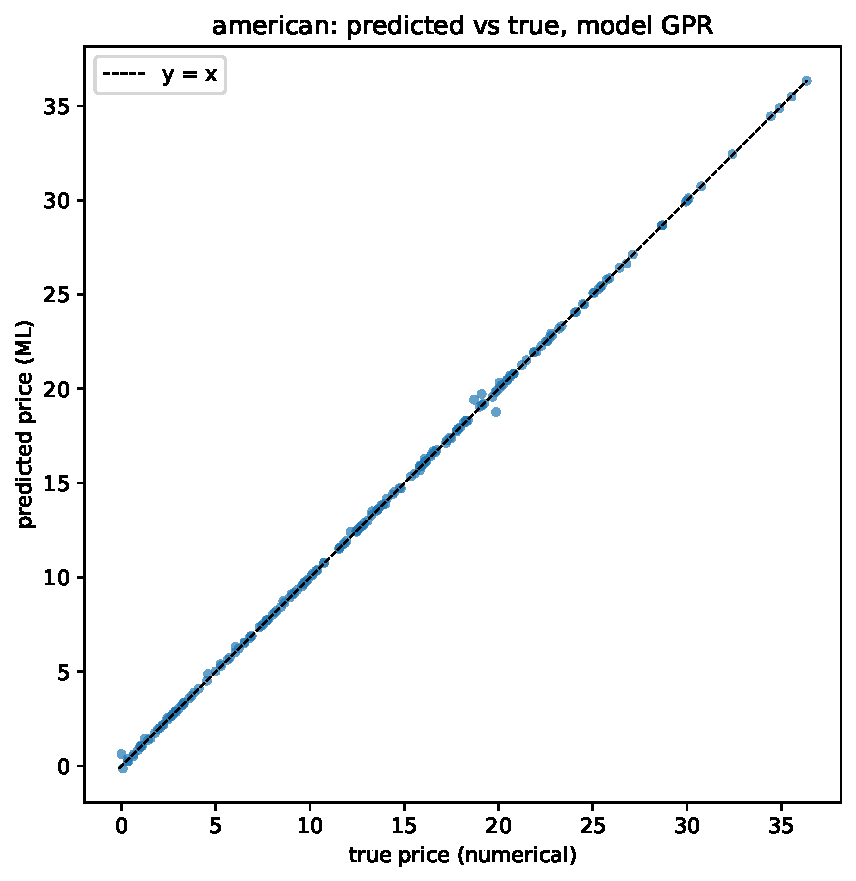
\includegraphics[width=0.46\textwidth]{ex2/figures/01_pred_vs_true_american_GPR.pdf}
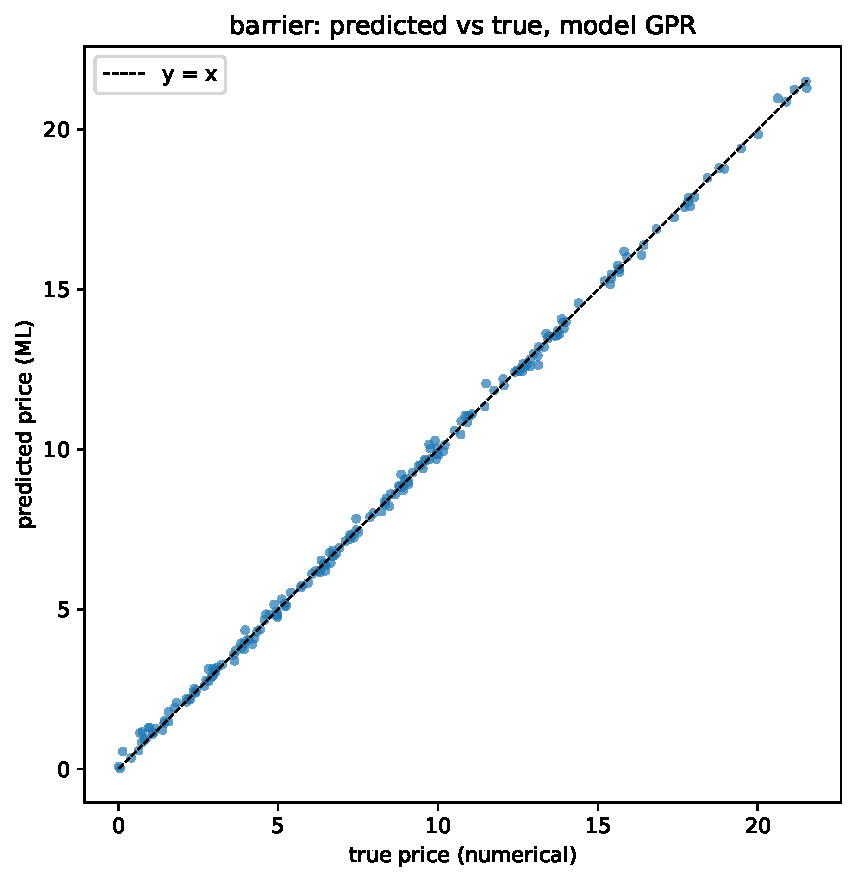
\includegraphics[width=0.46\textwidth]{ex2/figures/01_pred_vs_true_barrier_GPR.pdf}
\caption{Predicted versus true test-set prices for the GPR model: American
(left) and Barrier down-and-out Call (right); the dashed line is the identity.}
\label{fig:ml_pred}
\end{figure}

The aggregate numbers hide some structure. Split by contract type
(Table~\ref{tab:putcall}), the GPR error runs a little larger on puts than
calls, which fits the richer early-exercise behaviour of the American put. The
network is roughly even across the two. Either way the single pooled model
loses little by handling both. No-arbitrage checks (Table~\ref{tab:noarb})
confirm the surrogates mostly respect the price bounds. Predictions are
non-negative on essentially all test options, never exceed the spot ceiling for
calls and dip below intrinsic value only on a handful of deep contracts where
the unconstrained regressor overshoots by a few cents. None of these is enforced in training, so the small
violation rates are a fair picture of where a production system would want a
clamp. One bound is barrier-specific. A down-and-out call must weakly lose value
as the barrier $B$ rises toward spot, because knock-out grows more likely. We
test this by bumping $B$ by two points on each test option and checking the
predicted price does not rise. The GPR keeps the price monotone on $\BaMonoGPR\%$ of
cases and the NN on $\BaMonoNN\%$. At roughly three-quarters, the surrogate is not
production-safe in $B$, since neither model enforces the bound. A deployed pricer
would add a monotonicity constraint or a post-processing step such as isotonic
projection along the barrier. The check is cheap and finance-specific, the kind
of audit a learned pricer should pass before use.

\begin{table}[ht]
\centering
\footnotesize
\begin{minipage}[t]{0.49\textwidth}
\centering
\setlength{\tabcolsep}{4pt}
\begin{tabular}{llrrr}
\toprule
model & subset & MAE & RMSE & $R^2$ \\
\midrule
GPR & put ($90$)  & 0.063 & 0.140 & 0.99972 \\
GPR & call ($110$) & 0.047 & 0.122 & 0.99981 \\
NN  & put ($90$)  & 0.130 & 0.188 & 0.99949 \\
NN  & call ($110$) & 0.146 & 0.279 & 0.99899 \\
\bottomrule
\end{tabular}
\captionof{table}{American GPR and NN test errors split by put and call (subset
sizes in brackets).}
\label{tab:putcall}
\end{minipage}\hfill
\begin{minipage}[t]{0.49\textwidth}
\centering
\setlength{\tabcolsep}{3pt}
\begin{tabular}{llrrr}
\toprule
contract & model & ${<}\,0$ & ${<}$ intr. & ${>}$ bound \\
\midrule
American & GPR & 0.5\% & 2.0\% & 0\% \\
American & NN  & 1.0\% & 3.0\% & 0\% \\
Barrier  & GPR & 0\%   & n/a   & 0\% \\
Barrier  & NN  & 1.5\% & n/a   & 0\% \\
\bottomrule
\end{tabular}
\captionof{table}{Share of test predictions violating non-negativity, the
intrinsic-value floor (American) and the upper price bound.}
\label{tab:noarb}
\end{minipage}
\end{table}

\begin{table}[ht]
\centering
\footnotesize
\begin{tabular}{lrrr}
\toprule
dataset & mean MC SE & 90th-pct SE & GPR MAE \\
\midrule
Barrier Heston labels & 0.083 & 0.137 & 0.122 \\
\bottomrule
\end{tabular}
\caption{Monte Carlo noise of the barrier labels: mean and 90th-percentile
antithetic standard error against the GPR test MAE, which sits at the noise floor.}
\label{tab:mc_se}
\end{table}

\subsection{Discussion}
On the American surface the GPR reaches an $R^2$ all but equal to one, with a
typical error around five cents on prices that run from zero to forty and it
prices puts and calls equally well from a single model. On the barrier surface
the target is not the exact Heston price but a Monte Carlo estimate, so the test
residual mixes model error and label noise. The GPR MAE of $\BaGPRmae$ sits right at
the noise floor of those labels (mean standard error $\BaSEmean$, with a $90$th
percentile of $\BaSEpHi$). It has therefore reached about the best a surrogate can
do against noisy targets rather than coming within a tenth of a euro of the true price.
The network is an order of
magnitude cheaper to fit and to query, at the cost of two to three times the
MAE. It is the engine to reach for when latency dominates, with GPR as the
accuracy benchmark when it does not.

The speedups need one qualification. The column compares one already-trained
prediction against one fresh numerical pricing call, but training is a one-off
cost that we only repay after enough queries. The break-even count is
\[
N_{BE} = \frac{T_{\text{fit}}}{t_{\text{num}}-t_{\text{pred}}},
\]
training time over the per-query time saved, \emph{not} the number of training
samples divided by the speedup. With our timings this is about $\AmGPRbe$
American GPR queries, $\AmNNbe$ American NN queries, $\BaGPRbe$ Barrier GPR
queries and just over $\BaNNbe$ Barrier NN queries. Below those counts the numerical pricer is cheaper
if no model exists yet. Above them, which is the normal regime in production
where the same parameter range is queried thousands of times, the surrogate is
decisively faster. The exact break-even is hardware-dependent (these timings are
from the machine that produced the tables), but the ordering is robust: the
cheap-to-train network repays itself fastest, the expensive GPR needs the most
queries to amortise.

\clearpage
\section{Faster Euler Monte Carlo}

Every variant below estimates the same quantity, the discounted
expected payoff. Under Euler discretisation a geometric-Brownian path follows
$S_{t+\Delta t}=S_t+rS_t\Delta t+\sigma S_t\sqrt{\Delta t}\,\epsilon_t$ with
volatility $\sigma$ and $\epsilon_t\sim N(0,1)$ and the option value is
approximated by $m^{-1}\sum_{i=1}^{m} f(\widehat S_{i,n})\,e^{-rT}$, where $m$ is
the number of paths, $f$ the payoff and $\widehat S_{i,n}$ the simulated price at
the final step $n$ of path $i$. We split the
computation into three blocks: generating the innovations, simulating the
security paths and evaluating the discounted payoff. Each improvement below
touches just one block and leaves the priced quantity alone. It only makes the
estimator faster or cuts its variance.

\subsection{The variants}
\begin{enumerate}[label=\roman*., itemsep=1pt]
  \item V0 is the baseline, a doubly nested Python loop with one
  scalar normal per step per path.
  \item V1 keeps the same arithmetic Euler step but vectorises across
  paths, so the path loop disappears into a NumPy broadcast. This changes only
  the \texttt{SecurityPath} block.
  \item V2 adds antithetic variates, drawing $N/2$ normals $Z$ and
  using $Z$ and $-Z$, so the symmetric part of the noise integrates exactly.
  This changes the \texttt{OptInnovations} block.
  \item V3 replaces the arithmetic step with the log-Euler step
  $\log S_{t+\Delta t}=\log S_t+(r-\tfrac12\sigma^2)\Delta t+\sigma\sqrt{\Delta t}\,Z$,
  which is exact for geometric Brownian motion and removes the discretisation
  bias of the arithmetic scheme.
  \item V4 swaps the pseudo-random draws for a scrambled Sobol
  low-discrepancy sequence mapped through the inverse normal CDF, again acting on
  the innovations.
\end{enumerate}
For Heston we also use a full-truncation Euler scheme. Writing
$v_t^+=\max(v_t,0)$, the variance and log-price updates the code applies are
\[
v_{t+\Delta t}=v_t+\kappa(\theta-v_t^+)\Delta t
  +\eta\sqrt{v_t^+}\sqrt{\Delta t}\,Z^v_t,
\]
\[
\log S_{t+\Delta t}=\log S_t+\left(r-q-\tfrac12 v_t^+\right)\Delta t
  +\sqrt{v_t^+}\sqrt{\Delta t}\,Z^S_t,
\]
with correlated shocks $Z^S_t=\rho Z^v_t+\sqrt{1-\rho^2}\,\epsilon_t$ and
$Z^v_t,\epsilon_t\sim N(0,1)$. Flooring the variance at zero inside the square
roots is what keeps them well defined under discretisation. It changes the
numerics, not the risk-neutral Heston model.

\subsection{Vanilla benchmark}
Table~\ref{tab:euler} prices a European call with $S_0=K=100$, $T=1$, $r=0.03$,
$\sigma=0.25$, whose Black-Scholes value is $\BSMref$. The scalar baseline runs
only $2{,}000$ paths, the most that is tractable in pure Python. Vectorisation
buys the dominant gain, close to two orders of magnitude per path while reaching
ten times as many paths. Antithetic variates roughly halve the runtime by
drawing $N/2$ shocks instead of $N$. For this one fixed seed the signed pricing
error also falls, from $\EulerErrVone$ for V1 to $\EulerErrVtwo$ for V2, but a
single signed
error is not a variance. The true variance reduction is the one in
Figure~\ref{fig:conv}, where the RMS error is averaged over $20$ seeds. Log-Euler
shaves a little more time and removes the small arithmetic bias. The Sobol variant is slower per run because the generator costs more than a
pseudo-random draw, but it converges faster in $N$, as Figure~\ref{fig:conv}
shows.

\begin{table}[ht]
\centering
\footnotesize
\setlength{\tabcolsep}{4pt}
\begin{tabular}{llrrrr}
\toprule
variant & description & price & error vs BSM & time (ms) & paths \\
\midrule
V0 & scalar loop, arithmetic Euler & 11.286 & $-0.063$ & 471 & 2{,}000 \\
V1 & vectorised, arithmetic Euler  & 11.579 & $+0.231$ &  48 & 20{,}000 \\
V2 & V1 + antithetic               & 11.413 & $+0.065$ &  24 & 20{,}000 \\
V3 & V2 + log-Euler                & 11.412 & $+0.064$ &  20 & 20{,}000 \\
V4 & V3 + Sobol QMC                & 11.296 & $-0.052$ & 195 & 20{,}000 \\
\bottomrule
\end{tabular}
\caption{Vanilla European-call benchmark for the five variants against the
Black-Scholes truth $\BSMref$; V0 runs at fewer paths because the scalar loop is
slow.}
\label{tab:euler}
\end{table}

\begin{figure}[h]
\centering
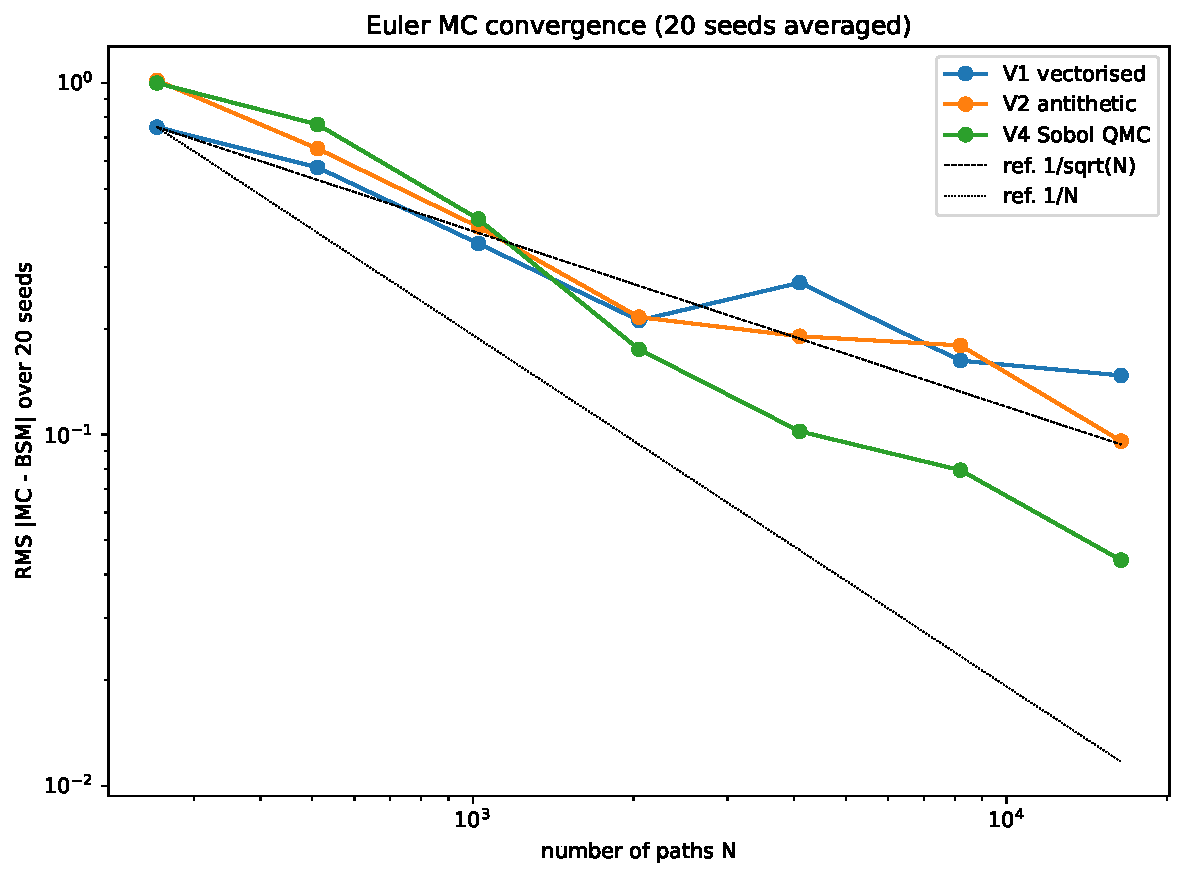
\includegraphics[width=0.74\textwidth]{ex3/figures/01_convergence.pdf}
\caption{RMS pricing error of the vectorised variants versus path count $N$,
averaged over $20$ seeds; scrambled Sobol (V4) breaks below the $1/\sqrt{N}$
reference.}
\label{fig:conv}
\end{figure}

\subsection{Heston benchmark}
For the Heston down-and-out call with $S_0=K=100$, $T=1$, $r=0.03$,
$v_0=\theta=0.04$, $\kappa=2$, $\eta=0.3$, $\rho=-0.5$, $B=80$ we compare the
scalar naive scheme against the vectorised full-truncation engine used in
Problem~2. The scalar version prices $1{,}000$ paths in $\HesScalarMs$ milliseconds, which
scales to roughly $\HesScaledMs$ milliseconds for the $10{,}000$ paths a stable
barrier price needs. The vectorised engine prices $10{,}000$ paths in
$\HesVecMs$ milliseconds. That is well over a hundredfold speedup and it is what makes the
$1000$-option ground truth of Problem~2 feasible in well under a minute rather
than tens of minutes.

\subsection{Discussion}
Vectorisation provides the dominant speedup, about two orders of magnitude in
CPU time. Antithetic variates then add a variance reduction worth roughly half a
path-count doubling. Log-Euler removes the small bias of the arithmetic scheme
at no cost. And flooring the variance keeps the Heston path well behaved under
discretisation. For Problem~2 we keep log-Euler with antithetic variates in the
vanilla pipeline and its full-truncation analogue in the barrier engine. One
caveat on Sobol. In this smooth, low-dimensional vanilla benchmark the scrambled
sequence does converge faster than pseudo-Monte Carlo over the range we tested,
but there is no such guarantee for the discontinuous, path-dependent barrier
payoff under Heston: that would need its own check and probably a path
construction that reduces the effective dimension. So we use Sobol for the
vanilla pricing and leave it out of the barrier engine.

\section{Author contribution}

All authors contributed equally.

\end{document}
